\documentclass[12pt,a4paper]{article}
\usepackage[spanish,es-tabla]{babel} % espanol
\usepackage[utf8]{inputenc} % acentos sin codigo
\usepackage[left=3.5cm,right=2cm,top=2.5cm,bottom=2cm,includehead,includefoot]{geometry}  %margenes segun pauta de la U
\usepackage{setspace}
\onehalfspacing %interlineado 1.5
\usepackage{graphicx}
\usepackage[usenames]{color}
\usepackage{amsfonts}
\usepackage{algpseudocode}
\usepackage{amsmath}
\usepackage{booktabs} %Rules en las tablas
\usepackage{listings}
\usepackage{xcolor}
\usepackage{afterpage}
\usepackage{float}
\usepackage{subfigure}
\usepackage{verbatim} %Comentarios con \begin end comment
\usepackage{csquotes}
\usepackage{datetime} %Para obtener formato a la fecha
\usepackage[backend=biber,style=alphabetic]{biblatex}%packages Bibliografia
\addbibresource{biblio.bib}%se carga el archivo
\usepackage{times} %font times new roman (?)
\usepackage{hyperref}
\hypersetup{
	colorlinks=false, %set true if you want colored links
	linktoc=all,     %set to all if you want both sections and subsections linked
	linkcolor=blue,  %choose some color if you want links to stand out
	pdfborder={0 0 0},
}


\newcommand{\grad}{$^{\circ}$}

\newcommand{\nombreTesis}{\textsc{sistema de evaluación y bio-feedback para Balance postural}}

\newdateformat{fecha}{%Método para obtener el mes y el año
	\monthname[\THEMONTH] \THEYEAR}

\DeclareLabelalphaTemplate{
	\labelelement{
		\field[uppercase,final]{shorthand}
		\field[uppercase]{label}
		\field[uppercase,strwidth=3,strside=left,ifnames=1]{labelname}
		\field[uppercase,strwidth=1,strside=left]{labelname}
	}
	\labelelement{
		\field{year}
	}
}

\pagestyle{headings}

\begin{document}

\thispagestyle{empty}
\vspace*{-2cm}
\hspace{-3cm}
\hbox{\vsize = 5cm
\vbox{\hsize = 11cm
\begin{flushleft}
	{\small{\bf UNIVERSIDAD CAT\'OLICA DEL MAULE}\\
		Facultad de Ciencias de la Ingenier\'ia\\
		Escuela de Ingenier\'ia Civil Inform\'atica}
\end{flushleft}}

\vbox{\hsize = 7cm
	\begin{flushright}
		{\small{\bf PROFESOR GU\'IA}\\
			Mary Carmen Jarur\\
			\hspace{1cm}}
	\end{flushright}}
}
\vspace{5.5cm}

\begin{center}
	{\Large {\bf \nombreTesis}}
	
	\
	
	\
	
	\small {\bf H\'ECTOR GABRIEL PEREDO URBINA}\\
	
	
	\
	
	\
	
	\textmd{Tesis para optar al\\ T\'itulo Profesional de Ingeniero Civil Inform\'atico}
	
	\vspace{4cm}
	\vfill{{\large {\sc Talca, \fecha\today }}}
	
\end{center} 

\pagebreak

%%%%%%%%%%%%%%%%%%%%% FIN  PORTADA     %%%%%%%%%%%%%%%%%%%%%%%%%%%


%%%%%%%%%%%%%%%%%%%%% PORTADA COMISION    %%%%%%%%%%%%%%%%%%%%%%%%

\thispagestyle{empty}

\begin{center}
	{\small {\bf UNIVERSIDAD CATÓLICA DEL MAULE}}\\
	\small {\bf FACULTAD DE CIENCIAS DE LA INGENIERÍA}\\
	\small {\bf ESCUELA DE INGENIERÍA CIVIL INFORMÁTICA}
	
\end{center}
\vspace{1cm}

\begin{center}
	{\small {\bf TESIS PARA OPTAR AL}}\\
	\small {\bf AL TÍTULO PROFESIONAL DE INGENIERO CIVIL INFORMÁTICO}\\
\end{center}

\vspace{1cm}

\begin{center}
	\bf{ \nombreTesis}
	
	\
	
	\small {\bf  HECTOR GABRIEL PEREDO URBINA}\\
	
\end{center}

\vspace{1cm}

\begin{tabular}{l@{\hspace{1cm}}c@{\hspace{3cm}}l@{\hspace{1cm}}l}
	{\bf COMISI\'ON EXAMINADORA}&&{\bf FIRMA}&\\
	&&&\\
	PROFESOR GUÍA &&&\\
	MARY CARMEN JARUR MUÑOZ&&&\\
	\cline{2-3}
	&&&\\
	
	PROFESOR COMISI\'ON&&& \\
	DR. HERN\'AN MAUREIRA PAREJA&&&\\
	\cline{2-3}
	&&&\\
	
	PROFESOR COMISI\'ON&&& \\
	DR. MARCO ANTONIO MORA COFRE&&&\\
	\cline{2-3}
	&&&\\
	
	&&&\\
	NOTA FINAL EXAMEN DE T\'ITULO &&& \\
	\cline{2-3}
\end{tabular}
\vspace{.7cm}


\begin{center}
	\vfill{{\large {\sc Talca, \fecha\today }}}
\end{center}


\pagebreak

%%%%%%%%%%%%%%%%%%%%% FIN  PORTADA COMISION   %%%%%%%%%%%%%%%%%%%%%%

\thispagestyle{empty}
\tableofcontents %Indice de Contenidos
\thispagestyle{empty}
\listoffigures
\thispagestyle{empty}
\listoftables

\thispagestyle{empty}
\pagebreak
\setcounter{page}{1}

\let\stdsection\section
\renewcommand\section{\newpage\stdsection}



\section{Introducción}
La comprensión de las dinámicas y patrones de movimiento humano, se facilitan enormemente con el apoyo de tecnologías adecuadas, que permitan medir, registrar y analizar variables cinemáticas. Particularmente, el estudio del movimiento humano (Kinesiología) depende hoy en día de las facilidades tecnológicas que ofrece la electrónica (sensores, microcontroladores, sistema de adquisición de señales) y las ciencias de la computación (procesamiento, análisis y posterior reporte adecuado de  variables cinemáticas y cinéticas).  

Las soluciones tecnológicas que hoy existen, no solo permiten realizar el seguimiento (‘tracking’) y representación gráfica, sino que además facilitan la representación en tiempo real de las variables de interés, conformando con esto los denominados sistemas de Bio-feedback (retroalimentación de señales biológicas). Aunque existen alternativas adecuadas para estos fines, poseen el inconveniente en lo prohibitivo de su valor comercial junto con ser soluciones cerradas tanto en hardware como software, limita las funciones según las características propuestas por fabricante, hace prácticamente imposible la adición de nuevas funcionalidades y el uso para otros fines u obtención de la información capturada por los sensores incorporados.

Frente a este desafío, está la posibilidad de integrar tecnología para conseguir soluciones de menores costos, que permitan realizar investigación y al mismo tiempo explorar posibilidades de innovación tecnológica que den paso al desarrollo de tecnología generadora de impacto no tan sólo en el ámbito nacional probablemente de carácter global.

Particularmente, este proyecto propone desarrollar un sistema de integración hardware-software que permita el registro del comportamiento pendular de la posición bípeda quieta (variables de posición y velocidad angular en el tiempo), habilitando funciones de bio-feedback que permitan replicar evaluaciones de balance postural.

\subsection{Objetivos Generales}
Diseñar e implementar un prototipo de software-hardware basado en un microcontrolador Arduino y un sensor de velocidad angular y acelerometría de 3 ejes, para el registro y representación gráfica del centro de masa y bio-realimentación.

\subsection{Objetivos Específicos}
\begin{itemize}
	\item Integrar microcontrolador Arduino con sensor (giroscopio-acelerómetro).
	\item Diseñar sistema que permita el registro y visualización de todas las variables cinemáticas (posición y velocidad angular) del centro de masa. 
	\item Construcción de un sistema que facilite mediante bio-realimentación la posición del centro de presión (proyección del centro de masa).
\end{itemize}	

\subsection{Contribución Esperada}

El desarrollo del sistema permitirá medir y registrar el comportamiento del centro de masa y su respectiva proyección (centro de presión) durante la posición bípeda quieta, al mismo tiempo que realimentará la señal como mecanismo de evaluación de balance postural e implementación de biofeedback.

El principal alcance de la propuesta es la posibilidad de contar con una solución abierta, que facilita la importación de todos los registros además del procesamiento de las señales recogidas de las evaluaciones, permitiendo además integrar la solución a otros sistemas.

El costo del sistema, respecto a las soluciones de mercado (Biodex- Balance SD), es bajo, lo que le da viabilidad económica al proyecto, permitiendo además dejar el prototipo en operación en el Laboratorio de Biomecánica. 

Desde el punto de vista disciplinar (Ciencias de la Ingeniería), este proyecto materializa trabajos de investigación y colaboración transdisciplinario entre la Facultad de Ingeniería y la Facultad de Salud de la UCM. Además posiciona a los Ingenieros Informáticos como profesionales capaces de adecuarse a diferentes contextos mediante soluciones tecnológicas.

\subsection{Organizaci\'on de la Tesis}
\textcolor{red}{falta}


\section{Estado del Arte}

Más de un tercio de la población mayor de 65 años notifica algunos problemas con el balance o deambulación. Los pacientes con trastornos neurológicos o musculo-esqueléticos son aún más propensos a tener problemas de equilibrio que afectan a su movilidad. La complejidad del control del equilibrio es resultado  de muchos tipos diferentes de problemas que necesitan la evaluación clínica sistemática para un tratamiento eficaz.
El control del equilibrio es complejo e implica el mantenimiento de posturas \cite{mancini_relevance_2010}, mantener el movimiento y recuperar el equilibrio. El control de balance consiste en controlar el centro de masa del cuerpo entre los límites de estabilidad. Las evaluaciones clínicas del equilibrio pueden ayudar a evaluar el riesgo de caídas y/o determinar las causas de los trastornos del equilibrio subyacente. 
La mayoría de las escalas de valoración del equilibrio funcional evaluar caída el riesgo y la necesidad de rehabilitación equilibrio, pero no diferenciar los tipos de déficits de la balanza . Un enfoque de sistema para la evaluación clínica equilibrio puede diferenciar diferentes tipos de trastornos del equilibrio y un enfoque fisiológico puede determinar los mecanismos subyacentes sensoriomotoras contribuye a equilibrar trastornos. Las medidas objetivas de equilibrio valiéndose de medios informáticos y sensores inerciales portátiles pueden traer más precisión, exactitud y sensibilidad que las pruebas de equilibrio clínicas.

\textcolor{red}{Agregas mas referencias y algo relacionado con mi solucion}


\subsection{Estándares Estabilometría Clínica}
La estabilometría corresponde al estudio del Centro de Presión (COP) para determinar deficiencias posturales que perjudican el Balance.

\subsubsection{Mediciones} Existen estándares respecto a las características necesarias para la medición del COP \cite{scoppa_clinical_2013}.

Varias declaraciones sobre la cuestión sigue siendo objeto de debate de la normalización estabilometría fueron acordados por el ISPGR (International Society for Posture and Gait Research).
Se definió un conjunto de características metrológicas para las plataformas estabilométricas.
Basándose tanto en la práctica y verificación experimental se acordó que, para obtener una apropiada precisión y sensibilidad:
\begin{itemize}
	\item El intervalo de adquisición no debe ser inferior a 25s.
	\item La frecuencia de muestreo debe ser de al menos 50 Hz.
	\item Estándares Técnicos:
	\begin{table}[H]
		\centering
		\label{table:mediciones}
		\begin{tabular}{|c|c|}			
			\hline \textbf{Variable} & \textbf{Valor} 	\\ 
			\hline Exactitud 	& $>$ 0.1 mm 		\\ 
			\hline Presición 	& $>$ 0.05 mm 		\\ 
			\hline Resolución 	& $>$ 0.05 mm 		\\ 
			\hline Ancho Frecuencia & 0.01–10 Hz	\\ 
			\hline 			
		\end{tabular}
		\caption{Estándares Técnicos Mediciones}
	\end{table}	  
\end{itemize}

\subsubsection{Instrumentos} Entre instrumentos de medición utilizados para el estudio del Balance estan incluidos:

\begin{itemize}
	\item \textbf{Kistler:} Es un Gold Standard  en lo referente a estabilometría\cite{donath_testing_2012}, es una plataforma de fuerza de dimensiones
	0,4m por 0,6m que consta de cuatro 	transductores piezoeléctricos, situados en las esquinas. Estos transductores son capaces de medir las fuerzas de reacción del suelo en los planos verticales medio-lateral (x), antero-posterior (y) tal como muestra la Figura (\ref{fig:Kistler}).

\begin{figure}[H]
	\centering
	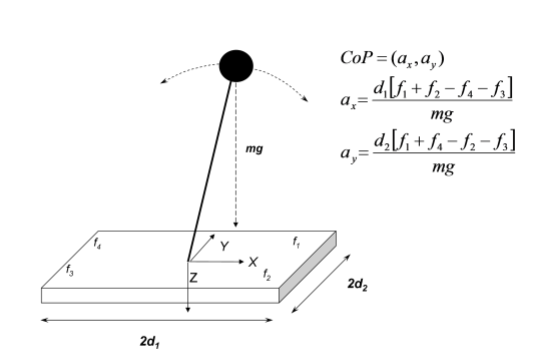
\includegraphics[width=0.7\linewidth]{images/Kistler}
	\caption{Calculo COP Kistler}
	\label{fig:Kistler}
\end{figure}

\item \textbf{Balance SD?:} 
\textcolor{red}{Falta}
	 
\end{itemize}

\subsection{IMU's}
\textcolor{red}{Falta}

\subsection{Estudio del Balance usando Sensores}
Recientemente, los sensores de movimiento ``weareables'' se han desarrollado para la robótica, industria aeroespacial y en las mediciones biomédicas se han utilizado para medir el control del balance\cite{mancini_relevance_2010}. Estos sensores, con transferencia inalámbrica de datos , tienen el potencial de superar los principales inconvenientes de coste, tamaño y ubicación limitado de las pruebas computarizadas , así como permitir la medición objetiva de la oscilación postural y movimientos durante la ejecución de tareas.

Desde que se inicio la experimentación de sistemas de biofeedback para el control postural, los sistemas de tipo táctil y audio han recibido mucha menos atención que la retro-alimentación visual.
Sin embargo, en los últimos años, el interés en sistemas táctiles y de audio para el control de la postura ha sido renovada, en parte debido a los avances en la tecnologías de procesamiento y detección de movimiento en tiempo real junto con las nuevas tendencias en dispositivos portátiles inalambricos que pueden ser usados durante todos los días. 
En 2001, Wall et al. \cite{giansanti_energetic_2009} 

En particular, Chiari et al. mostró, utilizando una plataforma de fuerza, que los sujetos mejoraron el equilibrio aprovechando el ABF (Audio Biofeed-back) y que ésta mejora fue mayor cuanto más grave era el desorden sensorial del sujeto. Otros estudios demostraron cómo este ABF mejora la estabilidad de la postura de los participantes con pérdida vestibular bilateral permitiendo gran cantidad de correcciones posturales.

\textcolor{red}{Falta Referencia!!!}

Los acelerómetros y/o giroscopios han sido exitosamente utilizados \cite{mancini_relevance_2010} para el seguimiento de movimiento,  detección de caídas, y para la medición de control de balance sólo recientemente se han utilizado también para la activación dispositivos de biofeedback vibro-táctil o ABF. Hasta ahora los acelerómetros y giroscopios no se han utilizado de forma regular en la investigación de la postura pese al éxito de la propuesta del dispositivo de ABF.


\section{Marco Teórico}

\subsection{Protocolo de Comunicación $\mathbf{\mathrm{I^2C}}$}
Para la comunicación entre el Arduino y los Sensores, y debido a la limitante del tipo de protocolo usados por el MPU6050, se debe utilizar protocolo de comunicación $I^2C$.

El protocolo $I^2C$ fue desarrollado en 1982 por Philips Semiconductors (hoy NXP Semiconductors) para la comunicación interna entre circuitos integrados como por ejemplo juegos de CD y televisiones.

Las principales características del protocolo de Comunicación $\mathrm{I^2C}$ \cite{I2C} son:
\begin{itemize}
	\item Solo dos líneas para la comunicación son necesarias; una línea para la información serial (SDA) y otra para el reloj serial (SCL).
	
	\item Cada dispositivo conectado al bus es direccionado por software por un ID único y usando relación Esclavo/Maestro todo el tiempo.
	
	\item Posee un sistema de detección de colisiones lo que permite usar el modo multi-maestro previniendo la corrupción de los datos si dos o mas maestros comienzan a transferir datos de forma simultánea.
	
	\item Orientado a transferencias de datos en 8-bit de forma bi-direccional pueden ser realizadas hasta los 100 kbit/s en el modo Estándar, hasta 400 kbit/s en el modo Rápido, hasta 1 Mbit/s en el modo Mas Rápido, o hasta 3.4 Mbit/s en el modo de Alta-Velocidad.
	
	\item En el chip de filtrado se rechazan los picos en la línea de datos del bus de preservar la integridad de datos.
	
	\begin{figure}[H]
		\centering
		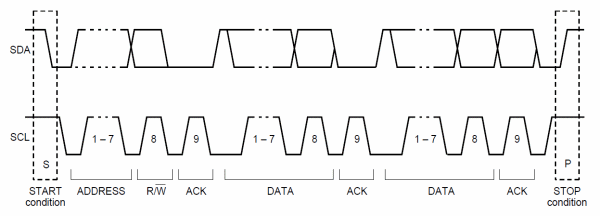
\includegraphics[width=0.9\textwidth]{images/Diagrama_I2C}
		\caption{Diagrama $\mathrm{I^2C.}$}
		\label{fig:diagramaI2C}
	\end{figure}
\end{itemize}

\subsection{Sistemas Coordenados}
Toda la información obtenida debe estar asociado según un sistema específico de coordenadas, que sirva de referencia clara para la interpretación y comprensión de la información.

Para ello fueron considerados los principales sistemas utilizados para referenciar los ejes coordenados según los distintas situaciones:
\begin{itemize}
	
	\item \textbf{Planos anatómicos} 
		\subitem \textbf{Plano Sagital:}
		 Se toma de referencia el cuerpo humano trazando línea una  vertical de referencia que teóricamente cruza el cuerpo por la parte media y central, a modo de plomada imaginaria, esta línea ayuda en la distinción de miembros o elementos en el «lado izquierdo» o «lado derecho».
		 \subitem \textbf{Plano Frontal:} Forma un ángulo recto con los planos sagitales. En un ser humano, el plano medio coronal divide el cuerpo en posición de pie en dos mitades (frontal y dorsal, o anterior y posterior) mediante una línea imaginaria que corta ambos hombros.

	\begin{figure}[H]
		\centering
		\includegraphics[width=0.5\textwidth]{images/planosAnatomicos}
		\caption{Planos Anatómicos}
		\label{fig:sagital}
	\end{figure}

	\item \textbf{Ejes del sensor:} Los ejes contenidos en el sensor son expresados en coordenadas X, Y ,Z, en donde según la orientación del sensor cualquiera de sus ejes puede ser paralelo a la gravedad de la tierra, que apunta hacia el centro de esta.
\end{itemize}

\subsection{Sistema microelectromecánico (MPU6050)}
El sistema Microelectromecánico (MEMS) MPU6050\cite{MPU6050}, es un dispositivo capaz de medir la velocidad angular y fuerza de gravedad gracias a estar compuesto por Giroscópico y Acelerómetro ambos de 3 ejes, el hecho de poseer estos 2 sensores de movimiento indica que existen al menos 6 grados de libertad para utilizar al momento de obtener las mediciones provenientes de éste.

La tecnología utilizada MEMS patentada por InverSense, en el caso del giroscopio consiste en masas vibratorias verticalmente alineadas las cuales son usadas para crear un chip de bajo costo.

El MPU6050 está diseñado para realizar seguimiento (Tracking) gracias a que posee un bajo consumo, es de bajo costo, y cumple con los requisitos de los teléfonos inteligentes, tabletas y sensores portátiles \cite{MPU6050}.
La transmisión de datos con el microcontrolador es realizada únicamente mediante el protocolo I2C, el cual requiere de 2 líneas de conexión una para el envío de datos (SDA) y otra para el clock (SCL), las cuales varían dependiendo del modelo de microcontrolador, junto con la alimentación que consiste en la línea de voltaje (VCC) y conexión a tierra (GND).

El acelerómetro incluido mide el movimiento lineal respecto a cada uno de sus tres ejes ver Figura (\ref{fig:MPU6050}), es decir la aceleración percibida por el movimiento y esta es expresada en proporción a la fuerza de gravedad (veces de g).

El giroscopio mide la rotación alrededor de cada uno de los ejes ver Figura (\ref{fig:MPU6050}), es decir la velocidad angular expresada en \grad/seg.

\begin{figure}[H]
	\centering
	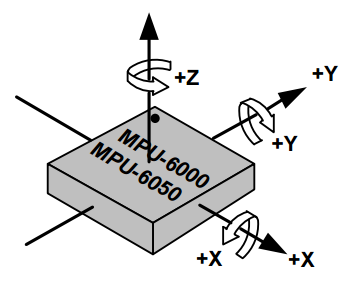
\includegraphics[scale=0.5]{images/MPU6050}
	\caption{Diagrama MPU6050}
	\label{fig:MPU6050}
\end{figure}

\subsubsection{Características Técnicas}

\begin{itemize}
	
	\item \textbf{Rango:} Poseen un rango configurable ambos sensores incluidos, tanto acelerómetro como giroscopio, el rango nos indica el dominio sobre el cual son adquiridos los datos, más concretamente los valores máximos y mínimos donde fluctúan la información obtenida.
	
	\item \textbf{Sensibilidad:} La sensibilidad describe la mínima variación medible, es decir la razón de cambio entre una variable entrante y el resultado de la variable saliente.
	
	\begin{table}[H]
		\centering
		\label{table:caracteristicasSensor}
		\begin{tabular}{|c|c|c|c|}
			\hline
			\multicolumn{2}{|c|}{Acelerómetro} &\multicolumn{2}{|c|}{Giroscopio}   \\
			\hline
			Rango (g)        & Sensibilidad (LSB/g)  & Rango (\grad/seg)     & Sensibilidad (LSB/\grad/seg)\\ \hline
			$\pm 2$     &  16384 & $\pm 250 $  	& 	131      	\\ 
			$\pm 4$     &  8192  & $\pm 500 $ 	& 	65.5     	\\
			$\pm 8$     &  4096  & $\pm 1000$  	& 	32.8       	\\
			$\pm 16$    &  2048  & $\pm 2000$   & 	16.4      	\\ 
			\hline
		\end{tabular}
		\caption{Características de los sensores LSB: Bit Menos Significativo}
	\end{table}
	
	\item \textbf{Variables:} Las variables entregadas por el Acelerómetro consiste en la aceleración lineal percibida en cada eje expresada en veces de g, y en el Giroscopio corresponde  a la velocidad angular dada por la variación de los grados en un instante de tiempo al girar sobre cada eje.
	
	\item \textbf{Frecuencia de Muestreo:} Nos describe la cantidad de datos que pueden ser obtenidos en un intervalo de tiempo, a su vez nos describe la diferencia de tiempo entre cada dato obtenido.
	
	\item \textbf{Resolución:} Consiste en la mínima variación generada en la variable medida y la cual los sensores son capaces de informar.
	
		\begin{table}[H]
			\centering
			\label{table:resolucionSensor}
			\begin{tabular}{|c|c|c|c|}
				\hline
				\multicolumn{2}{|c|}{Acelerómetro} &\multicolumn{2}{|c|}{Giroscopio}   \\
				\hline
				Rango (g)        & Resolución ($\Delta$LSB/g)  & Rango (\grad/seg)     &  Resolución ($\Delta$LSB/(\grad/seg))\\ \hline
				$\pm 2$     &  $6.10351562e^{-5}$   &$\pm 250 $ 	& 	$7.633587786e^{-3}$ 	\\ 
				$\pm 4$     &  $1.22070313e^{-4}$  	&$\pm 500 $ 	& 	$1.526717557e^{-2}$    	\\
				$\pm 8$     &  $2.44140625e^{-4}$ 	& $\pm 1000$  	& 	$3.048780488e^{-2}$		\\
				$\pm 16$    &  $4.88828125e^{-4}$   & $\pm 2000$    & 	$6.097560976e^{-2}$     \\ 
				\hline
			\end{tabular}
			\caption{Resolución de los sensores}
		\end{table}
	
\end{itemize}

\subsubsection{Configuración de MPU6050}
Por defecto el MPU6050 viene configurada con los parámetros básicos para realizar la captura de información, lo cual puede perfectamente ser útil según sea el caso de estudio, pero si se desea que los sensores operen en rangos específicos y/o los datos capturados por de los sensores sean obtenidos a frecuencias específicas se debe comprender como llevar a cabo la configuración en cada uno de los registros internos presentes, el mapa de los registros \cite{MAPREGISTER} proporcionado  en el sitio de InverSense es buena guía para entender cómo se realiza esta labor.
\newline En el interior del MPU6050 se encuentran más de 70 registros cada uno de 8 Bit, para la configuraciones listadas a continuación se deben ser usados solo algunos pocos.
\begin{itemize}
	\item \textbf{Configurar frecuencia muestreo:} Para obtener la cantidad de muestras que se obtendrán finalmente ``En Teoría'' se calcula usando la ecuación: 
	
	\begin{equation} 
		\label{eq:sampleratediv}
		Sample Rate = \frac{Gyroscope Output Rate}{(1 + SMPLRT\_DIV) }
	\end{equation}
	
	En la ecuación (\ref{eq:sampleratediv}) factores, tales como la velocidad del puerto serial pueden influir en el resultado, pero cambiando los datos almacenados en el registro \textbf{SMPRT\_DIV}, con valores entre 0 y 255, el valor de $Gyroscope Output Rate$ depende directamente del estado del filtro pasa-bajo, en caso de estar desactivado, el valor de $Gyroscope Output Rate$ sería 8Khz, en cambio sí está activado el $Gyroscope Output Rate$ tomaría el valor de 1Khz con lo cual haciendo los cálculos necesarios al estar desactivado el filtro pasa-bajo la frecuencia de muestreo variará entre las 8000 y 31 muestras/seg de forma teórica, al contrario en caso de estar activado el filtro, la fórmula para el cálculo de la frecuencia de muestreo fluctuaría entre las 1000 y 3.9 muestras/seg, por cada uno de los 6 datos obtenibles.
	
	Nota: Hay que tener en consideración que el valor obtenido para la frecuencia de muestreo es válido principalmente para el giroscopio, ya que para el acelerómetro se maneja con su propia frecuencia de que es siempre de 1Khz por ende si la frecuencia de muestreo es mayor a 1Khz se pueden repetir valores en la salida del acelerómetro.
	
	\item \textbf{Configurar Giroscopio:} El registro GYRO\_CONFIG permite el cambio de los rangos para la obtención de la velocidad angular, con lo cual aumentamos o disminuimos de forma inversa la sensibilidad del Giroscopio. En el interior de este registro específicamente en los bits 3 y 4 del registro deben ser ingresados los valores en binario de los números 0, 1, 2 o 3 para configurar los cuatro rangos disponibles 250\grad/seg, 500\grad/seg, 1000\grad/seg y 2000\grad/seg. respectivamente.
	
	\item \textbf{Configurar Acelerómetro:} La configuración para el rango del acelormetro se realiza de forma similar, solo que en cambio el utilizado el registro ACCEL\_CONFIG, en donde también en los bits 3 y 4 se deben ingresar los valores en binario de 0, 1, 2 o 3 que representarán $\pm 2g$, $\pm 4g$, $\pm 8g$, $\pm 16g$ respectivamente.
	
\end{itemize}

\subsubsection{Obtención mediciones Giroscopio y Acelerómetro}
Luego de realizar la configuración de los registros del MPU6050, se deben leer ciertos registros para la obtención de la información del movimiento registrado por los sensores inerciales:

\begin{itemize}
	\item \textbf{Obtención de la Velocidad Angular:} Para obtener la variación del ángulo por unidad de tiempo medida por el giroscópico, deben ser leídos 6 registros en donde son usados por cada eje medible 2 registros de 8 bit,
	
	\begin{table}[H]
		\centering
		\label{table:registrosgyro}
		\begin{tabular}{|l|l|c|l|c|}
			\hline
			\textbf{Eje} & \textbf{Registro} & \textbf{Dirección (Hex)} & \textbf{Registro} & \textbf{Dirección (Hex)} \\ \hline
			X            & GYRO\_XOUT\_H     & 0x43                     & GYRO\_XOUT\_L     & 0x44                     \\ \hline
			Y            & GYRO\_YOUT\_H     & 0x45                     & GYRO\_YOUT\_L     & 0x46                     \\ \hline
			Z            & GYRO\_ZOUT\_H     & 0x47                     & GYRO\_ZOUT\_L     & 0x48                     \\ \hline
		\end{tabular}
		\caption{Registros mediciones Giroscopio}					
	\end{table}
	
	Posteriormente de ser leídos ambos registros de cada eje estos deben ser sumados usando aritmética binaria en donde el valor obtenido del primer registro leído le es aplicado un corrimiento de 8 bit para luego sumar el segundo obtenido, además se utiliza el complemento a 2 para la obtención de valores negativos, que genera como dato resultante un valor de entre aproximadamente $\pm 2^{15}$, este valor resultante debe ser dividido según la sensibilidad asociada a el rango escogido del giroscopio, para transformar el dato RAW del giroscopio y obtener la información física en (\grad/seg).
	
	\item \textbf{Obtención de la Aceleración:} Para obtener la información del acelerómetro al igual que en Giroscopio deben ser leídos los 6 pertenecientes a las mediciones:

	\begin{table}[H]
		\centering
		\label{table:registrosaccel}
		\begin{tabular}{|l|l|c|l|c|}
			\hline
			\textbf{Eje} & \textbf{Registro} & \textbf{Dirección (Hex)} & \textbf{Registro} & \textbf{Dirección (Hex)} \\ \hline
			X            & ACCEL\_XOUT\_H     & 0x3B                     & ACCEL\_XOUT\_L     & 0x3C                     \\ \hline
			Y            & ACCEL\_YOUT\_H     & 0x3D                     & ACCEL\_YOUT\_L     & 0x3E                     \\ \hline
			Z            & ACCEL\_ZOUT\_H     & 0x3F                     & ACCEL\_ZOUT\_L     & 0x40                     \\ \hline
		\end{tabular}
		\caption{Registros mediciones Acelerómetro}					
	\end{table}				
					
	Para luego unir los registros y usar el complemento a 2 acorde a cada eje, cada uno de estos valores deben ser divididos según el rango escogido, que determina la sensibilidad a usar para obtener la información física de la aceleración.
	
	\begin{figure}[H]
		\centering
		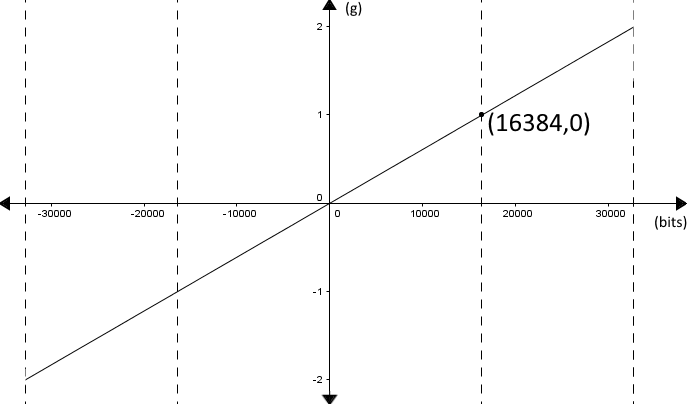
\includegraphics[scale=0.6]{images/curvacalibracion}
		\label{fig:curvacalibracion}
		\caption{Ejemplo curva calibración $\pm 2g$}
	\end{figure}
	
\end{itemize}

\subsection{Microcontroladores Arduino}
Arduino\cite{ARDUINO} es una plataforma de hardware de código abierto, basada en una sencilla placa con entradas y salidas, analógicas y digitales, con un entorno de desarrollo basado en el lenguaje de programación C++, donde sus principales características son:
\begin{itemize}
	\item \textbf{Bajo Coste:} Las placas Arduino son relativamente de bajo coste comparadas con otras plataformas microcontroladoras Handy Board, Basic Stamp\textregistered. La versión menos cara del módulo Arduino puede ser ensamblada a mano, e incluso los módulos de Arduino preensamblados cuestan menos de 50\$.
	\item \textbf{Multiplataforma:} El software de Arduino se ejecuta en sistemas operativos Windows, Macintosh OSX y GNU/Linux. La mayoría de los sistemas microcontroladores están limitados a Windows.
	\item \textbf{Entorno de programación simple y claro:} El entorno de programación de Arduino es fácil de usar para principiantes, pero suficientemente flexible para que usuarios avanzados puedan aprovecharlo también. Para profesores, está convenientemente basado en el entorno de programación Processing, de manera que estudiantes aprendiendo a programar en ese entorno estarán familiarizados con el aspecto y la imagen de Arduino.
	\item \textbf{Código abierto y software extensible:} El software Arduino está publicado como herramientas de código abierto, disponible para extensión por programadores experimentados. El lenguaje puede ser expandido mediante librerías C++, y la gente que quiera entender los detalles técnicos pueden hacer el salto desde Arduino a la programación en lenguaje AVR C en el cual está basado. De forma similar, puedes añadir código AVR-C directamente en tus programas Arduino si quieres.
	\item \textbf{Código abierto y hardware extensible:} El Arduino está basado en microcontroladores ATMEGA8 y ATMEGA168 de Atmel. Los planos para los módulos están publicados bajo licencia Creative Commons, por lo que diseñadores experimentados de circuitos pueden hacer su propia versión del módulo, extendiéndolo y mejorándolo. Incluso usuarios relativamente inexpertos pueden construir la versión de la placa del módulo para entender cómo funciona y ahorrar dinero.

\end{itemize}


\subsection{Framework QT}
Qt es un Framework basado en C++, tiene disponibilidad multiplataforma- escritorio, móvil y sistemas embebidos.
Posee las bibliotecas bases de C++  junto a librerías y herramientas de desarrollo propias de Qt, en donde se incluye IDE Qt Creator, y herramientas de productividad .
El entorno de desarrollo (IDE) del framework de C++ Qt  es Qt Creator en donde se incluyen las herramientas para la administración de los ficheros .h y .cpp usados en C++ junto con las opciones de compilación, ejecución y depuración del software.


\section{Desarrollo}
\subsection{Introducción}

A partir de la noción general que intrínsecamente cada uno posee de un estudio del balance y complementado con las ideas de herramientas o técnicas ya existentes que intentan solventar mediante diversos puntos de vista la problemática.

Usando de referencia principalemente los equipamientos disponibles en el Laboratorio de Bio-mecánica que sirvieron de base para el desarrollo de la solución Hardware-Software fueron la plataforma de fuerza Kistler 9286b \cite{KISTLER} y balance SD, que en ambos casos dan una representación del movimiento del centro de masa/presión y utilizando la representación entregada se ideó una solución que opera de forma análoga a los dispositivos que ya son utilizados en el laboratorio con un software que permita entregar información de manera similar a lo que entregan estos sistemas, para aprovechar los conocimientos de los usuarios con el fin de disminuir la curva de aprendizaje del sistema implementado para que estos comprendan el software sin demasiado entrenamiento y a su vez la transición sea más satisfactoria para estos.

En lo referente a Hardware se utilizó un sensor inercial MPU6050, el cual será puesto en el sujeto de prueba en una posición aproximada al centro de masa que éste a su vez captura la información del movimiento generado por el sujeto y lo trasmite al microcontrolador Arduino en donde se recibe y traduce la información obtenida del sensor además de transmitir al ordenador los datos obtenidos utilizando variables físicas, tanto aceleración y velocidad angular en donde finalmente el software del ordenador recibe la información y realiza el procesamiento para obtener el ángulo y desplazamiento junto con brindar la opción de efectuar análisis específicos de la información utilizando interfaces gráficas sencillas.


\begin{figure}[H]
	\centering
	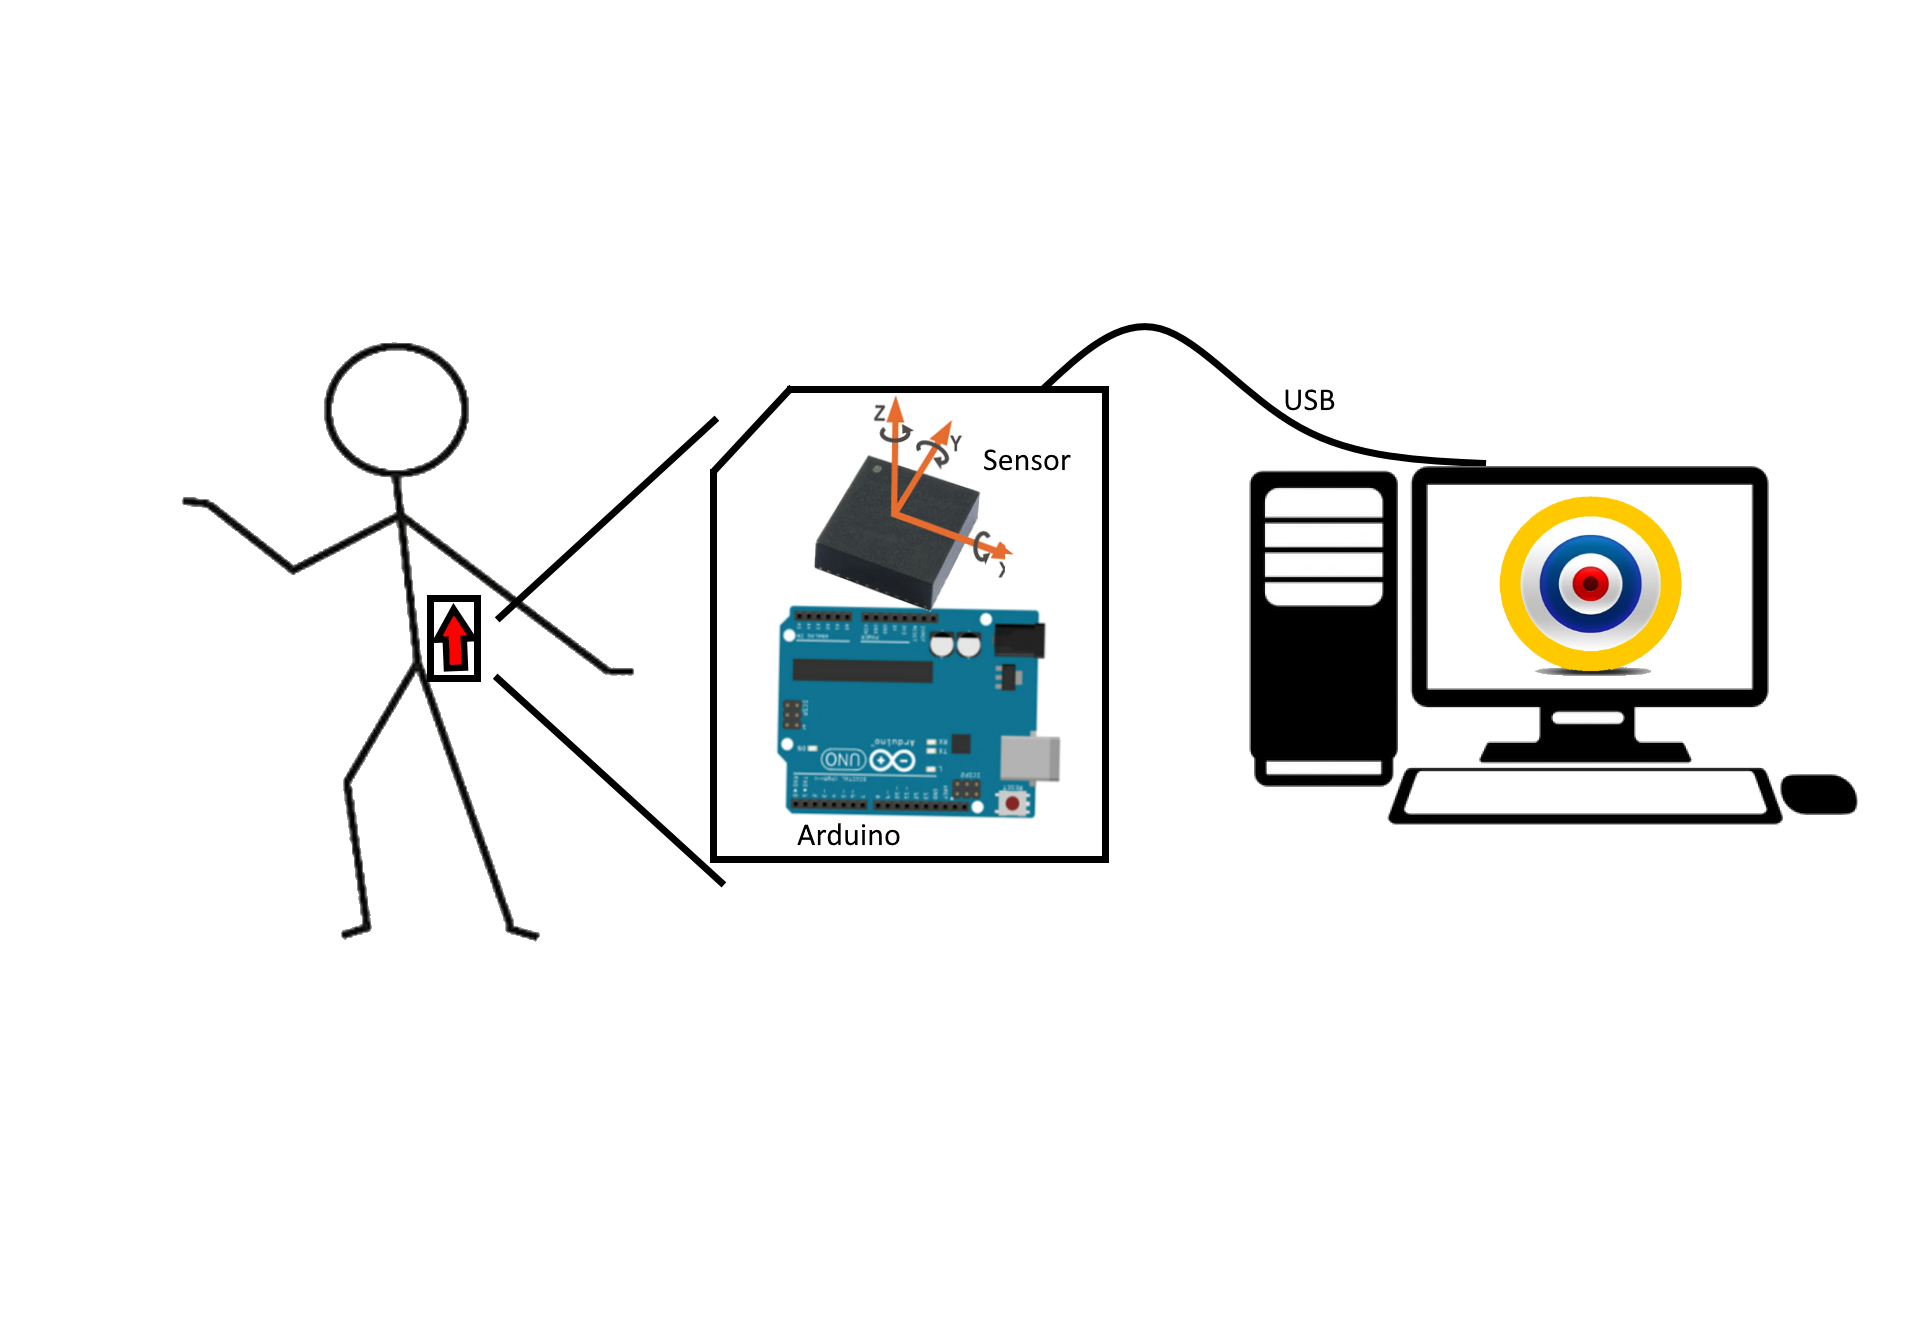
\includegraphics[scale=0.15]{images/diagrama_sistema}
	\caption{Diagrama Sistema}
	\label{fig:diagramasistema}
\end{figure}

\subsection{Programación en Arduino}
Uno de los primeros pasos en el desarrollo de la solución consiste en utilizar el IDE de Arduino para realizar la programación inicial del microcontrolador, en donde se debe configurar las direcciones de los registros internos del MPU6050 usados, junto con la configuración inicial, además de definir el formato de envío para desplegar los datos por el puerto serial.
En el Loop de ejecución de Arduino se obliga a configurar el MPU6050, mediante la escritura de comandos en el puerto serial, para ajustar las configuraciones de los sensores a conforme las necesidades del usuario ver Figura (\ref{fig:arduinocode}), para dar comienzo a la escritura serial de Arduino hacia PC.

\begin{figure}[H]
	\centering
	\includegraphics[scale=0.5]{images/diagramacodigoarduino}
	\caption{Diagrama Código Arduino}
	\label{fig:arduinocode}
\end{figure}

Existen 4 parámetros a ser configurados de forma obligatoria Frecuencia de Muestreo, Filtro pasa bajo, rango Acelerómetro y rango Giroscopio, antes de comenzar con la lectura de las de la información registros.
Para configurar los 4 parámetros requeridos debe ser recibida una cadena por el puerto serial en donde se analiza e interpretan los valores a utilizar para cada configuración. 
Una vez se completa la configuración se procede a la lectura de los registros para obtener los valores RAW tanto acelerómetro como giroscopio para finalmente enviar mediante comunicación serial el valor resultante expresado en su unidad física correspondiente al ser dividido por la sensibilidad según el rango previamente configurado.


\subsection{Cálculo Ángulo} 
Para efectos de análisis o representación final, a partir de las variaciones de aceleración y velocidad angular detectadas por los sensores existe la opción de calcular el ángulo, que es un indicador equivalente a la inclinación que ha realizado el sujeto.

Para ello existen distintos métodos usando la información obtenida, tales como:


\subsubsection{Cálculo Ángulo con Acelerómetro} Si es utilizado acelerómetro como inclinómetro este nos entrega el ángulo con gran exactitud pero al ser producida cualquier variación en la aceleración en cualquiera de sus 3 ejes de medición que no sea producto tan solo de la fuerza gravitacional será interpretada como un cambio de aceleración, lo cual genera medida erráticas debido a los cambios de aceleración constantes que son generados al girar/mover la IMU.
Para los cálculos del ángulo como se muestra en el ejemplo para el cálculo de los ángulos Medio-Lateral ver ecuación (\ref{eq:calculoanguloXsensorvertical}) e Antero-Posterior ver ecuación (\ref{eq:calculoanguloYsensorvertical}) usando el sensor en posición vertical con la referencia hacia atrás.

\begin{figure}[H]
	\begin{equation}
	anguloML = \tan{\left(\frac{aceleracionX}{\sqrt{aceleracionZ^{2}+aceleracionY^{2}}}\right)}
	\label{eq:calculoanguloXsensorvertical}
	\end{equation}
	\begin{equation}
	anguloAP = \tan{\left(\frac{aceleracionZ}{\sqrt{aceleracionX^{2}+aceleracionY^{2}}}\right)}
	\label{eq:calculoanguloYsensorvertical}
	\end{equation}
\end{figure}

\subsubsection{Cálculo ángulo con giroscopio} 
En cambio, si utilizamos sólo el giroscopio a diferencia del acelerómetro, podemos realizar los cálculos del ángulo con mayor precisión pero al no tener una referencia clara del origen de la mediciones, es difícil de contrastar la información con el movimiento de un sujeto y dificulta enormemente la  interpretación esta información, además con el tiempo los datos capturados comienzan a acumular un pequeño error, a estos errores acumulados se les conoce como drift o deriva.

\subsection{Fusión de Datos Sensores}
La Fusión de Datos es un método para integrar señales provenientes de múltiples fuentes. Permite extraer información de varias fuentes diferentes para integrarlos en una sola señal o información.

Para el análisis del desplazamiento del centro de masa se requiere el cálculo del ángulo y para ello se usará la información proveniente de ambos sensores con el fin de obtener el ángulo lo más refinado posible, con este fin se estudiaron e implementaron 2 filtros que permiten una correcta integración de los datos de aceleración con velocidad angular.

\subsubsection{El Filtro Complementario}

En síntesis tenemos un acelerómetro que entrega ángulos con referencia en la posición del sensor, pero muy susceptible a la variación de cambios de aceleración del IMU y en cambio el giroscopio nos permite calcular el ángulo de manera exacta, pero si tener una clara referencia de la posición donde está el sensor. 

Para unificar la información proveniente de ambos sensores existe un filtro, que nació principalmente de la práctica, conocido como el Filtro Complementario \cite[Capítulo 3, p.~44]{TesisUSM}.
El filtro requiere un ángulo de punto de partida y para esto se utiliza el acelerómetro para recoger el ángulo inicial, ya que, al poseer la referencia de la gravedad, se puede tener obtener una mejor estimación para comenzar a realizar las iteraciones del filtro.
\newline
El Filtro complementario es ampliamente usado en unidades inerciales y sistemas de visión. Este filtro es en sí es un filtro de Kalman de estado estacionario para una cierta clase de problemas de filtrado.
Está compuesto por la una unión de dos filtros diferentes:
\begin{itemize}
	\item \textbf{Filtro Pasa-Bajo:} Se usa para eliminar las frecuencias altas del acelerómetro, por lo cual dejamos pasar bajo ciertas frecuencias, para eliminar el ruido detectado por el cambio de aceleración (vibración principalmente) en los ejes del acelerómetro.
	\item \textbf{Filtro Pasa-Alto:} Se aplica en las mediciones obtenidas por el giroscopio, para eliminar el drift acumulado en el tiempo, dejando pasar solo las de una frecuencia más alta.
\end{itemize}

\begin{figure}[H]
	\centering
	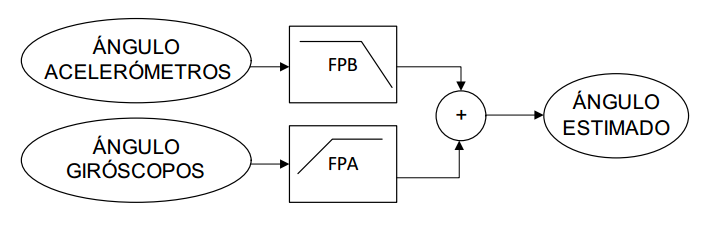
\includegraphics[scale=0.5]{images/FiltroComplementario}
	\caption{Diagrama Filtro Complementario}
	\label{fig:diagramafiltrocomplementario}
\end{figure}

Todo lo anterior queda descrito usando la siguiente Ecuación (\ref{eq:ecuacionFiltroComplementario}):

\begin{equation}
\label{eq:ecuacionFiltroComplementario}
anguloActual = (1-\alpha)*(anguloAnterior+\omega*dt)+(\alpha)*anguloAcelerometro
\end{equation}

En donde cada uno de las variables representa lo siguiente:
\begin{itemize}
	\item \textit{anguloAcelerometro:} El ángulo calculado mediante la aceleración obtenida por el Acelerómetro.
	\item $\omega$: Es la velocidad angular obtenida por el Giroscopio que hemos calculado previamente.
	\item \textit{dt:} Corresponde a la variación en segundos desde la última vez que se aplicó el filtro para calcular el ángulo.
	\item $\alpha$: Representa la contribución realizada por cada ángulo, Si $\alpha$ es igual 0 el cálculo del ángulo se realiza con el giroscopio en caso contrario $\alpha$ igual a 1 corresponde al ángulo del acelerómetro.
\end{itemize}

\subsubsection{Filtro de Kalman discreto}
El filtro de Kalman es un estimador lineal, insesgado y óptimo del estado de un proceso. En él se ha impuesto la condición de que el proceso a ser estimado es regido por una dinámica lineal y que el ruido que lo perturba es blanco y gaussiano. Aun cuando la condición del comportamiento probabilístico gaussiano del ruido se omite, el filtro de Kalman sigue siendo el mejor filtro recursivo lineal (error de menor varianza) e insesgado.

Su propósito es emplear las mediciones obtenidas en un período de tiempo que a su vez son afectadas por variaciones  aleatorias (ruido) junto con el conocimiento del comportamiento del sistema, para producir estimaciones que tiendan a estar más cerca del valor real del proceso en cuestión. Todas las mediciones y cálculos basados en modelos son aproximaciones en cierto grado, datos ruidosos provenientes de los sensores \cite[Capítulo 3, p.~45]{TesisUSM}. 

EL filtro de Kalman posee flexibilidad para ser utilizado tanto en tiempo continuo o en tiempos discretos. El modelo del filtro permite la flexibilidad para ser utilizado en éstos casos.

La principal diferencia es la notación que utilizada en cada uno de los casos.
Debido a que en la actualidad la mayoría de las aplicaciones de filtros es realizada en plataformas de tipo digital, y considerando el uso del filtro para la fusión de los sensores en este proyecto.

Filtro usado en Fusión de Datos \cite{mau_how_2005} 
El Filtro consiste en 2 estados Predicción y Actualización.

\textcolor{red}{LOREM IPSUM}

\begin{figure}[H]
	\centering
	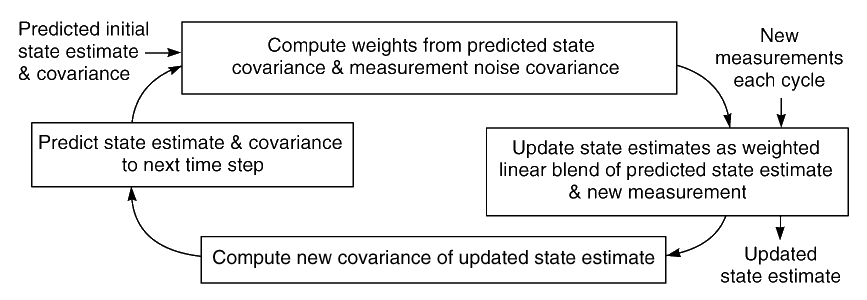
\includegraphics[scale=0.5]{images/kalman-filter.png} 
	\caption{Diagrama estados Filtro Kalman}
	\label{fig:diagramakalman}
\end{figure}


\subsubsection{Comparativa de Filtros}
Luego de la integración de los filtros en el Software es posible utilizar el deseado para la prueba, pero se deben tener en consideración las ventajas de usar o no el filtro razón por la cual se realizó una breve comparativa para ver el comportamiento entre el cálculo del ángulo sin utilizar filtros, usando filtro complementario y Kalman para la obtención durante la misma prueba.
Los resultados demuestran la gran corrección que realizan los filtros frente a el cálculo sin estos ver Figura (\ref{fig:AnguloXvsFiltros}).


\begin{figure}[H]
	\centering
	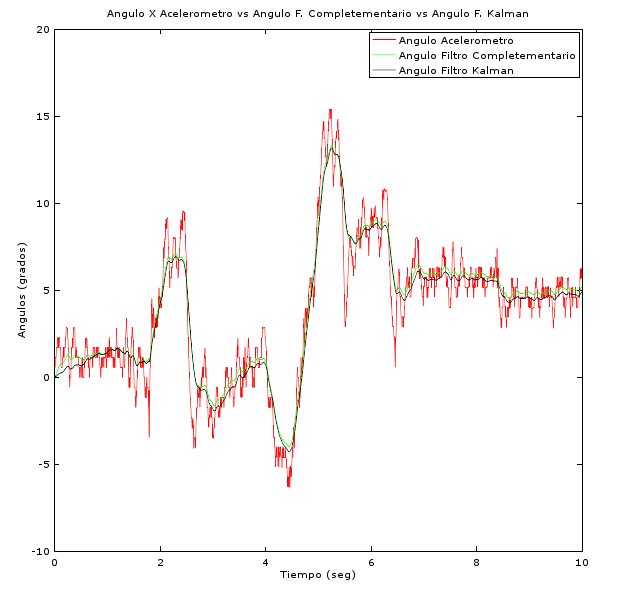
\includegraphics[scale=0.7]{images/angKalCom}
	\caption{Comparativa Angulo Acelerómetro vs Filtro Kalman vs Filtro Complementario}
	\label{fig:AnguloXvsFiltros}
\end{figure}

\subsection{Cálculo del Desplazamiento}
Basándonos en que la posición bípeda-quieta puede ser representada como un péndulo invertido, por lo tanto considerando la variación angular del movimiento pendular de un sujeto en las coordenadas antero-posterior y medio-lateral es aplicable la trigonometría para la obtención del desplazamiento.
Para el cálculo del desplazamiento usando la variación angular se consideraron los siguientes métodos. 

\subsubsection{Cálculo Proyección del Ángulo}
Para obtener la distancia proyectada en el eje horizontal, usando trigonometría tomando la altura $h$ como la distancia desde el suelo hasta donde fue puesto el sensor como el equivalente a la hipotenusa de un triángulo rectángulo, como se muestra en la Figura (\ref{fig:proyeccion}), se puede calcular usando la Ecuación (\ref{eq:proyeccion}), aplicando la función $\sin$ del ángulo $\alpha$ en grados obtenido mediante el filtro aplicado, junto con ponderar el valor obtenido por la altura $h$ (hipotenusa del triángulo), el valor resultante equivale a la distancia $d$ correspondiente al desplazamiento del centro de masa estimado, en la cual su unidad de medida es la misma usada para describir la altura $h$ en general centímetros.

\begin{figure}[H]
	\centering
	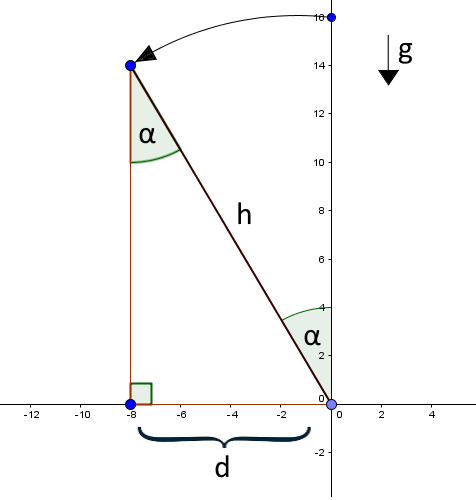
\includegraphics[scale=0.5]{images/calculoProyeccion}
	\caption{Ejemplo cálculo Proyección Angulo}
	\label{fig:proyeccion}
\end{figure}

\begin{equation}
	\label{eq:proyeccion}
	d=\sin(\alpha)*h
\end{equation}


\subsubsection{Cálculo del Recorrido Curvo}
La longitud del arco generado por el ángulo puede ser considerado un tipo de desplazamiento, por ello existe la opción de estudiarlo.

Calculando la longitud del arco formado desde donde comienza la medición hasta el ángulo $\alpha$ ver Figura (\ref{fig:recorridocurvo}) en grados a radianes y ponderando el valor obtenido por la altura $h$, tal como se muestra en la Ecuación (\ref{eq:recorridocurvo}).

\begin{figure}[H]
	\centering
	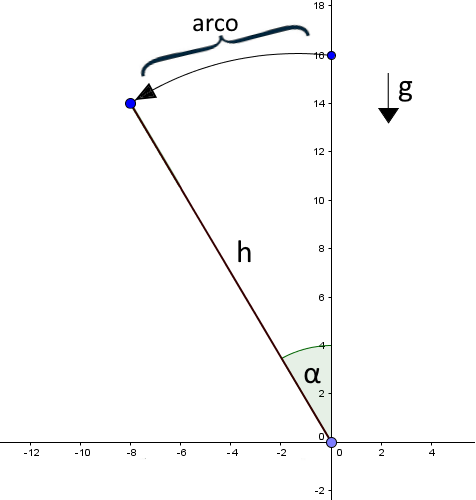
\includegraphics[scale=0.5]{images/calculoRecorridoCurvo}
	\caption{Ejemplo cálculo Recorrido Curvo}
	\label{fig:recorridocurvo}
\end{figure}

\begin{equation}
	\label{eq:recorridocurvo}
	d=\left(\frac{\alpha*2\pi}{360}\right)*h
\end{equation}

\subsubsection{Comparación Cálculo Recorrido Curvo vs Proyección}
Al comparar los métodos anteriormente mencionados para el cálculo del desplazamiento, estos se comportan de forma similar en ángulos pequeños, pero al aumentar el valor del ángulo se comienza diferenciar de forma exponencialmente el desplazamiento calculado por el recorrido curvo frente al obtenido por proyección, lo que nos da a concluir que ambos métodos entregan en ángulos pequeños desplazamientos similares, pero al aumentar el ángulo se comportan diferente.

Por lo tanto se debe tener en consideración al momento de escoger con que método se realizará el cálculo, ya que con ambos se puede interpretar el desplazamiento.

\begin{figure}[H]
	\centering
	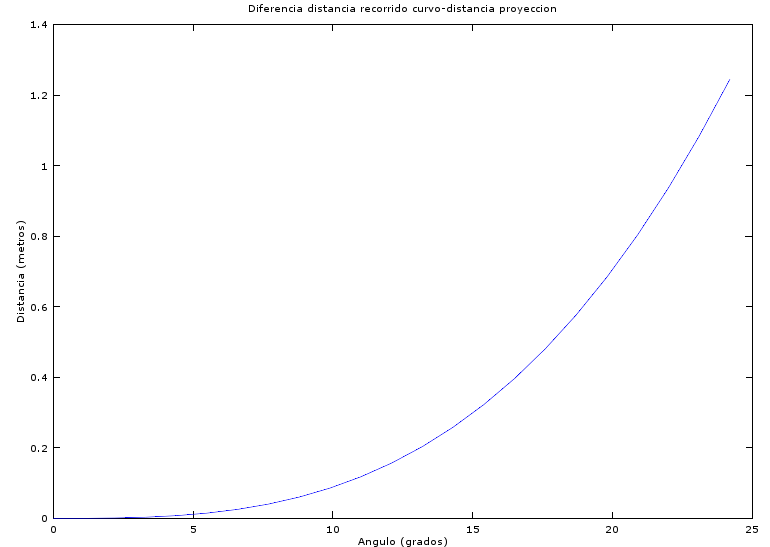
\includegraphics[scale=0.8]{images/DiferenciaRec-Pro}
	\caption{Ejemplo Diferencia distancia Recorrido Curvo - Distancia proyección}
	\label{fig:diferenciarec-pro}
\end{figure}


\subsection{Requisitos Funcionales}
\begin{itemize}
	\item El sistema debe ser capaz de describir mediante el estudio de variables cinemáticas (aceleración y velocidad angular), procesarlas y realizar análisis kinesiólogos (desplazamiento del Centro de Masa).
	\item El sistema debe ser capaz de representar en Tiempo Real el desplazamiento del centro de masa.
	\item El sistema debe permitir la generación de reportes, con todas las variables estudiadas y analizadas durante la prueba.
	\item El sistema debe permitir la configuración de los Sensores, ajustar su sensibilidad rango.
	\item Se debe permitir la configuración de las variables involucradas en cada pruebas a realizar, partiendo por la altura desde la que fue puesta el sensor, la orientación de éste, tiempo de prueba, etc.
	\item En lo referente a análisis de los gráficos de resultados, debe ser posible calcular estadísticos, como media, desviación estándar y junto con los valores máximos y mínimos.
\end{itemize} 

\subsection{Requisitos No funcionales}
\begin{itemize}
	\item El sistema debe presentar una interfaz clara y sencilla, tanto en el manejo, como para la presentación de resultados.
	\item El sistema debe tener un nombre representativo.
	\item El sistema debe permitir análisis usando los gráficos y mostrando los cambios (recortes o ajustes) en tiempo real.
\end{itemize}

\subsection{Resumen de Características}
\begin{itemize}
	\item \textbf{Configurable:} El software permite configurar la gran mayoría de opciones tanto velocidades de muestreo, Puerto Serial a utilizar, los rangos para la captura de información del movimiento, así como cantidad de datos que se representaran en pantalla, tamaños de los elementos a graficar, tiempos de prueba, limitar geométricamente el gráfico, entre otros.
	\item \textbf{Geometría Analítica} Se usó bastante la geometría analítica, para la generación y representación gráfica tanto de los objetivos en las pruebas, como para la intersección del movimiento realizado con cada uno de estos. De igual manera se utiliza la trigonometría para limitar el área del movimiento según el radio que sea definido para el examen.
	\item \textbf{Reportes:} Cada uno de los gráficos, los que despliegan las medidas tomadas o los que representan los resultados del ejercicio, pueden ser almacenados en muestras de cada uno de los gráficos, o también generar una imagen de estos.
	\item \textbf{Herramientas de Análisis Gráficas:} Ventanas desplegables acompañadas a un gráfico que permiten de forma interactiva seleccionar partes del gráfico, para analizar intervalos según se estime conveniente y a su vez obtener de este datos como, los valores máximos y mínimos, la media, desviación estándar de los datos, y en el caso del desplazamiento obtener la velocidad media del intervalo analizado.
\end{itemize}

\subsection{Codificación del Software}
Un parte importante del sistema es la interfaz que permite al usuario interactuar con el micro-controlador sin conocer más a fondo su funcionamiento,
con este propósito fue implementado utilizando en Framework QT(C++)\cite{QT} en su versión Open-Source, al estar basado en C++ en cuanto a estabilidad y rendimiento se refiere es una de las mejores opciones a tener en consideración.

El software permite la captura y procesamiento de información proveniente de la comunicación serial entre el micro-controlador Arduino y el ordenador,
El usar un framework como Qt facilita en gran parte la creación de interfaces gráficas, capa de funcionalidad que C++ no contiene por defecto, esto posibilita una rápida integración entre la parte lógica y visual del software a desarrollar.
Debido a el tipo de proyecto a implementar la metodología usada para el desarrollo fue el método ágil, al ser una solución de software con requisitos funcionales poco definidos, más que nada pautas del resultado esperado en donde el programador pasa a ser es el principal diseñador definiendo por sí mismo la distribución y comportamiento de los componentes del software.

En etapas tempranas del desarrollo se implementó una interfaz que se tan solo se comunicara con el puerto serial, pudiendo conectarse a este, y obtener la información que se encontrara disponible.
Durante el desarrollo se incluyeron más opciones para una visualización más agradable, junto con la parametrización de todos los elementos mostrados, permitiendo al usuario activar y desactivar opciones según sea el caso.

La comunicación serial entre el dispositivo-ordenador no solo es usada para leer los datos en el puerto, también es posible enviar los parámetros para realizar la configuración del sensor, para definir las opciones que consideradas más relevantes tales como: la frecuencia de muestreo, el uso del filtro Pasa-Bajo y los rangos tanto Acelerómetro como Giroscopio, usando una interfaz sencilla e intuitiva ver Figura (\ref{fig:ajustessensores}).

\begin{figure}[H]
	\centering
	\includegraphics[scale=0.6]{images/ajustesSensores}
	\caption{Ventana Ajustes Sensores}
	\label{fig:ajustessensores}
\end{figure}

Al momento de iniciar la aplicación si es que son detectados dispositivos en el puerto Serial se lanza la interfaz principal ver Figura (\ref{fig:mainwindow}), en donde se elige un paciente y la prueba a realizar.

\begin{figure}[H]
	\centering
	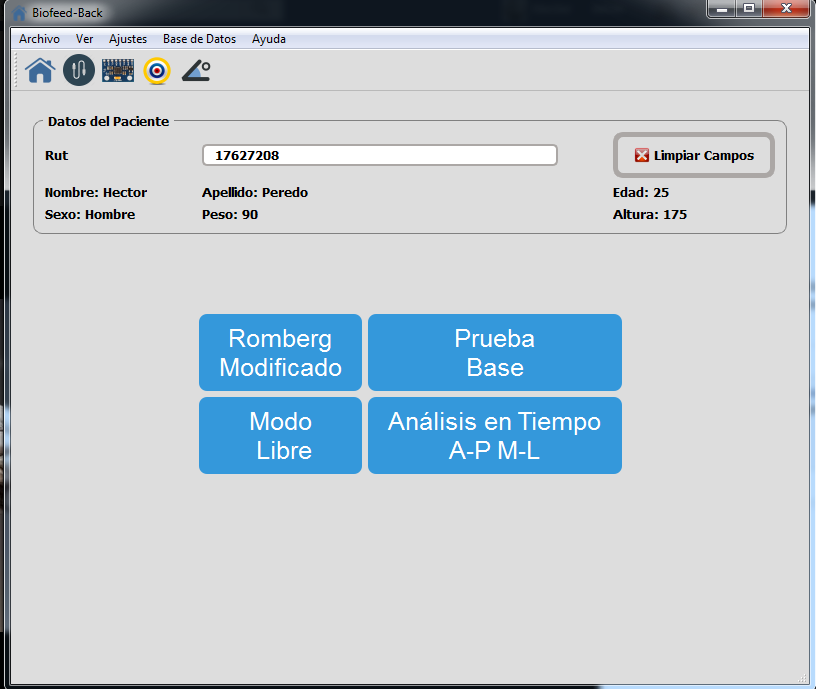
\includegraphics[scale=0.6]{images/mainwindow}
	\caption{Ventana Principal}
	\label{fig:mainwindow}
\end{figure}

Luego de seleccionada la prueba, según el tipo de prueba se permite configurar ciertos elementos, la interfaz fue pensada en ajustar la mayor cantidad de opciones sin sobrecargar demasiado ver Figura (\ref{fig:configurarPrueba}).

\begin{figure}[H]
	\centering
	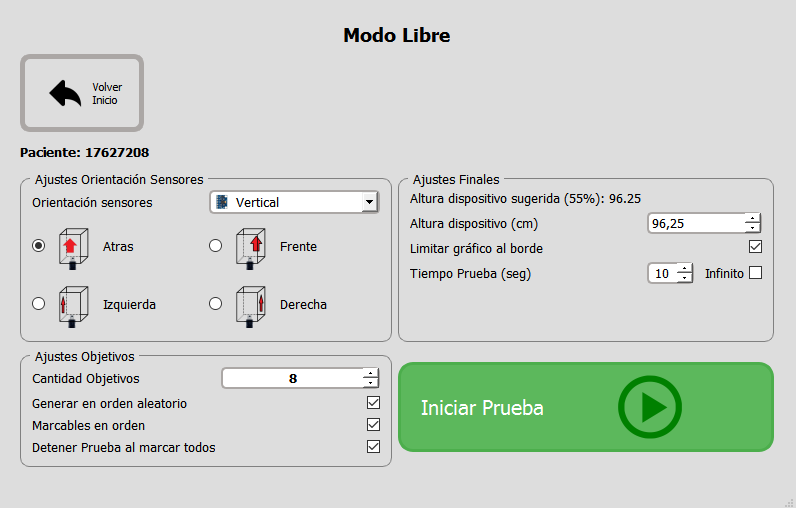
\includegraphics[scale=0.6]{images/configurarPrueba}
	\caption{Ventana Configuración Prueba}
	\label{fig:configurarPrueba}
\end{figure}

De entre los elementos configurables existen los siguientes

\begin{itemize}
	\item \textbf{Orientación Sensores:} Es una de las principales configuraciones a tener en consideración, debido a que define como está siendo situado el equipo, y a su vez como será analizada la información.
	Existen 2 categorías de orientación:
	\begin{itemize}
		\item \textbf{Horizontal:} En donde se puede definir si la referencia esta hacia adelante, atrás, izquierda o derecha, si esta orientación es seleccionada el cable siempre está conectado en la parte inferior del dispositivo.
		\item \textbf{Vertical:} Solo fueron considerados 2 modos, ya que de por si la orientación horizontal es poco práctica para los estudios del balance.
		Los modos disponibles son con la referencia arriba o abajo, considerando que el cable siempre sale hacia la derecha del dispositivo.
	\end{itemize}
	\item \textbf{Ajustes Objetivos:} En el gráfico principal se pueden desplegar objetivos para ser seguidos.
	\begin{itemize}
		\item \textbf{Cantidad de Objetivos:} Permite definir cuantos objetivos van a ser dibujados en pantalla, se debe tener en consideración los radios tanto de los objetivos, como del gráfico circular donde serán puestos, dado que si la cantidad de objetivos no es posible de dibujar, serán agregados la cantidad máxima posible sin que se intersecten.
		\item \textbf{Generar en orden Aleatorio:} Los objetivos pueden ser puestos en posiciones al azar dentro del gráfico o seguir una trayectoria circular.
		\item \textbf{Marcables en orden:} Define como se interacciona con los objetivos, si esta esta opción activada los objetivos parpadearán según el orden que fueron agregados permitiendo marcar solo uno, sino no parpadearán indicando que es posible marcar cualquier objetivo.
		\item \textbf{Detener prueba al marcar todos:} Como su nombre lo indica es definido si al pasar por todos los objetivos es finalizada la prueba o continua.
	\end{itemize}
	
	\item \textbf{Ajustes Finales} Son los ajustes referentes a si contara con un tiempo especifico para la prueba, a  y la opción de  para la representación.
	\begin{itemize}
		\item \textbf{Altura dispositivo:} La altura donde está puesto el dispositivo, que servirá para los cálculos de desplazamientos realizados.
		\item \textbf{Limitar el borde al gráfico:} Permite que la curva dibujada sobre el gráfico pueda salir o no del Radio Exterior de este.
		\item \textbf{Tiempo Prueba:} La cantidad de segundos que durará la prueba, o si esta se realizará de tiempo infinito.
	\end{itemize}
\end{itemize}

Nota: Algunos ajustes pueden interferir en el funcionamiento de otros, por ejemplo si es seleccionada la opción de Detener al marcar todos, pese a que el tiempo sea infinito la prueba terminará si se cumple la condición.

Luego de realizar la configuración y presionando el botón Iniciar Prueba, se procede a desplegar la información obtenida, en forma de gráficos.

\begin{figure}[H]
	\centering
	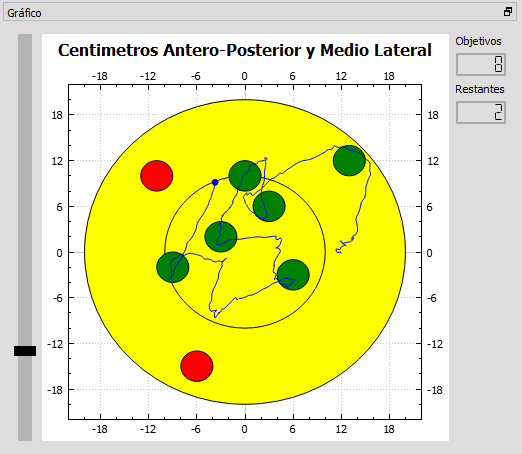
\includegraphics[scale=0.7]{images/graficoPrincipal}
	\caption{Gráfico de Prueba}
	\label{fig:graficoPrincipal}
\end{figure}


\begin{figure}[H]
	\centering
	\frame{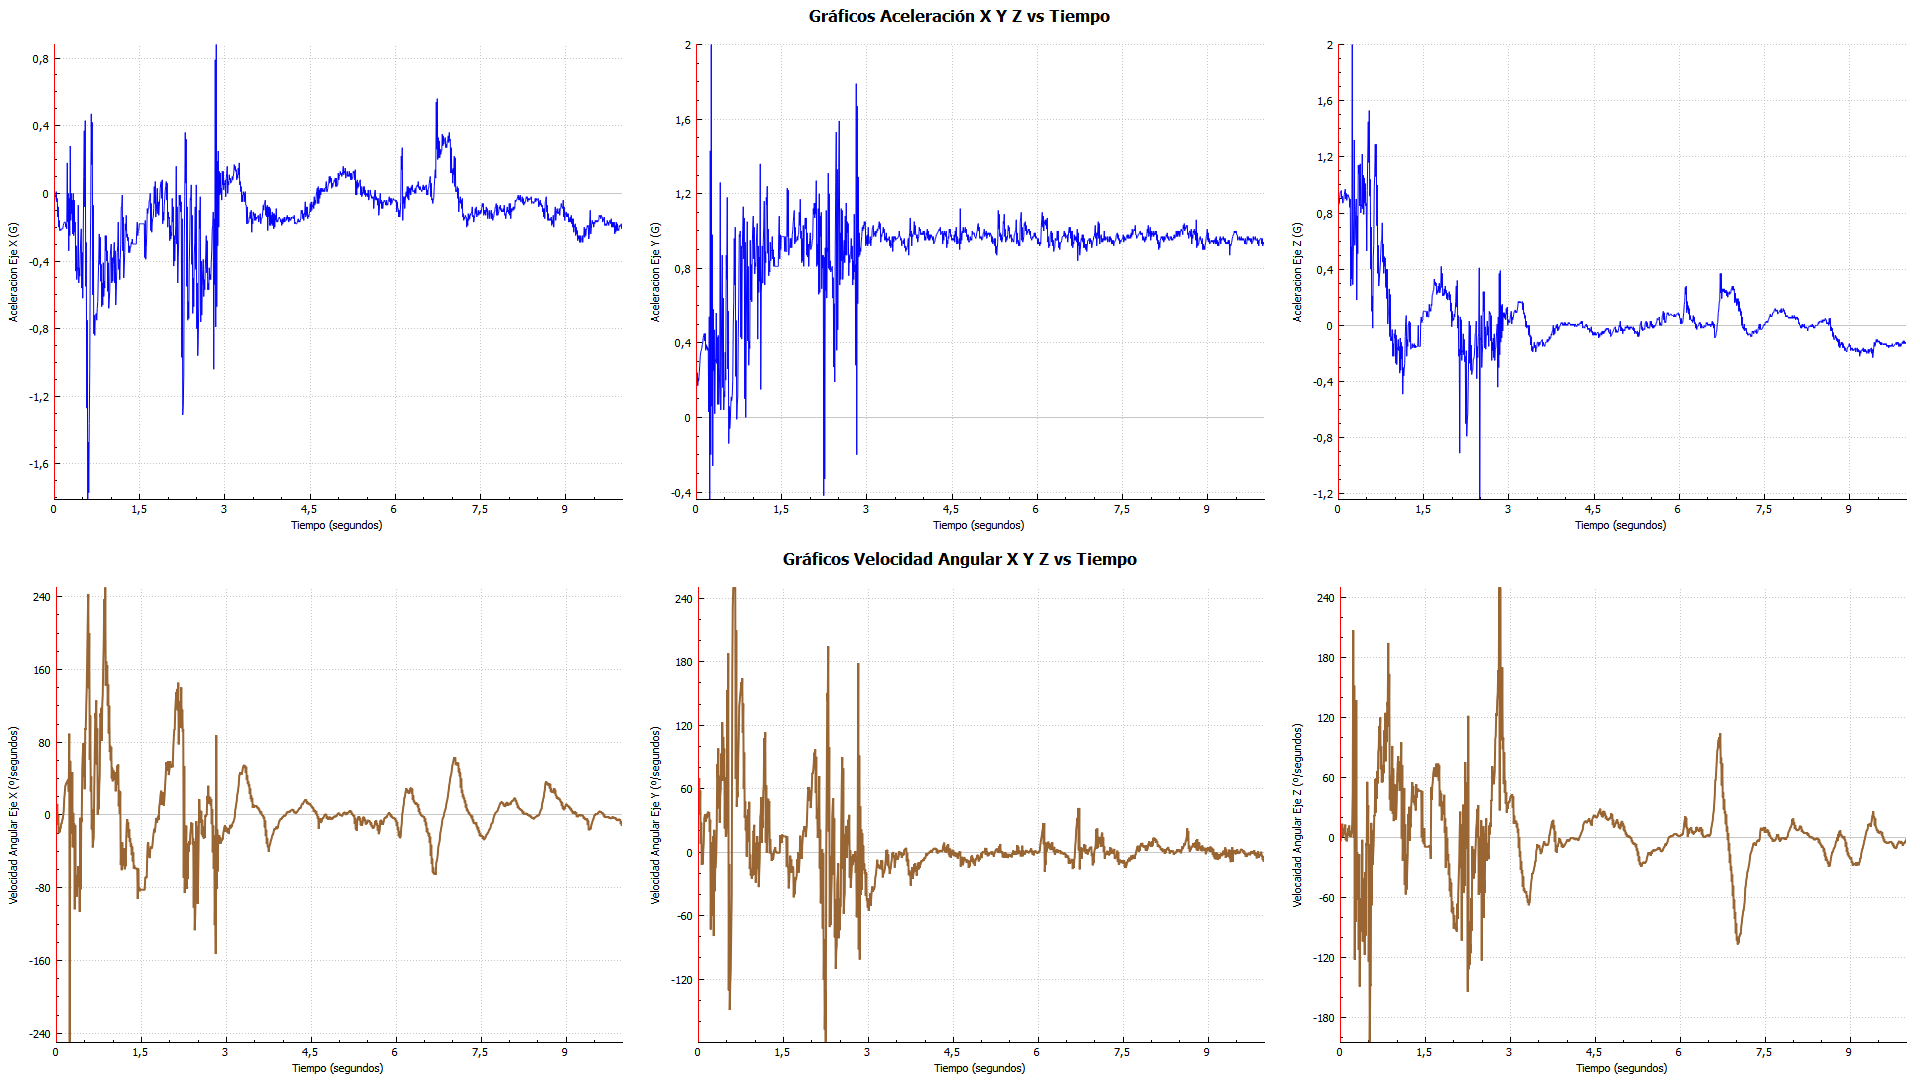
\includegraphics[scale=0.3]{images/graficosensores}}
	\caption{Gráficos de los sensores}
	\label{fig:Graficosensores}
\end{figure}

Finalmente para el análisis de la información se dispone de herramientas intuitivas que permiten seleccionar intervalos, para el cálculo de estadísticos de la prueba, media, máximos, mínimos, etc. ver Figura (\ref{fig:analsisGraficos}).

\begin{figure}[H]
	\centering
	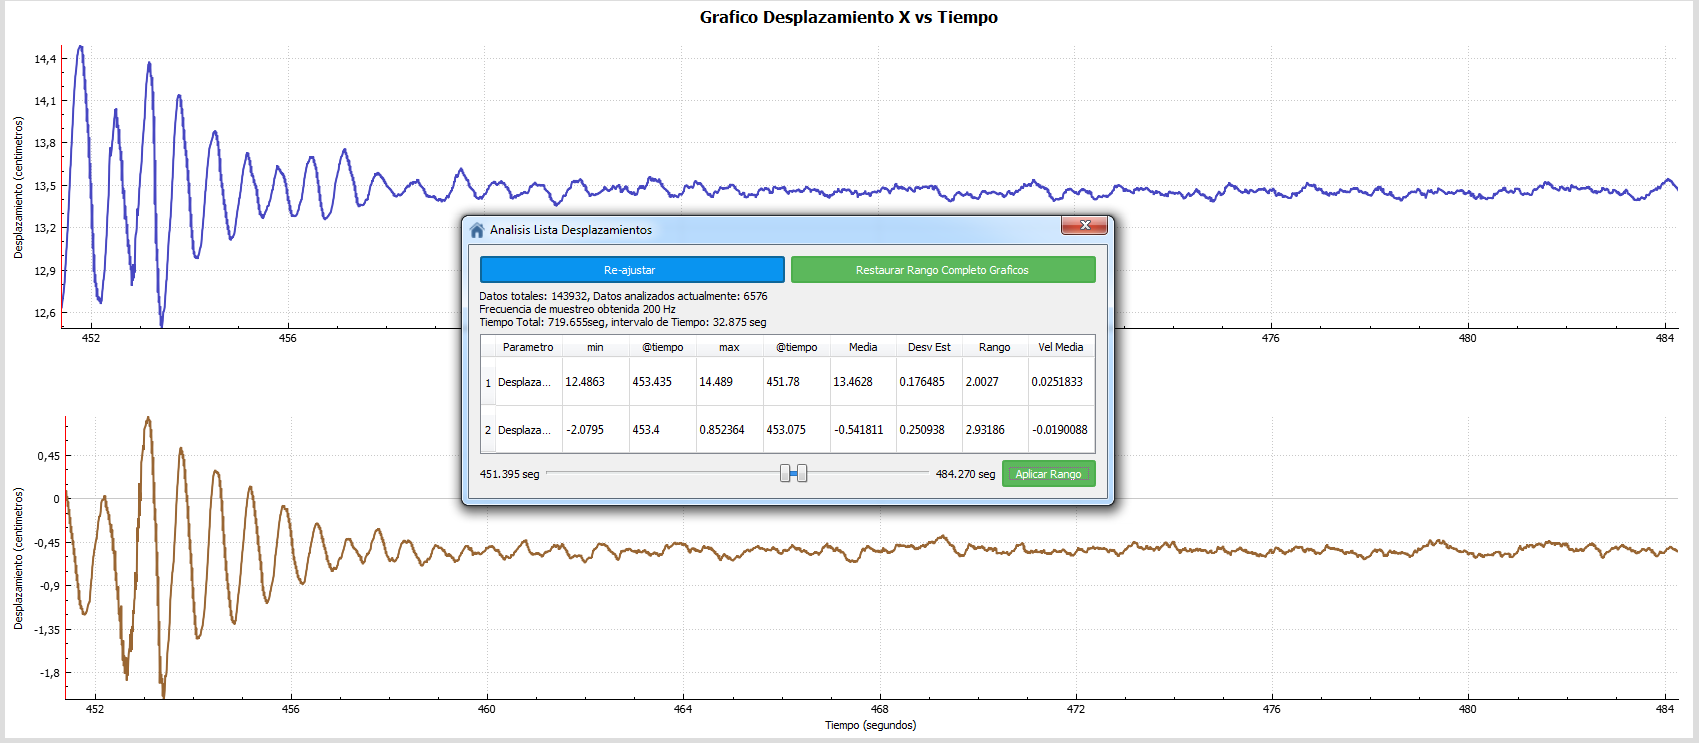
\includegraphics[scale=0.3]{images/analisisGraficos}
	\caption{Ejemplo Herramienta de Análisis}
	\label{fig:analsisGraficos}
\end{figure}


\subsection{Tests}
Contraste vs Plataforma de Fuerza Kistler
\begin{figure}[H]
	\centering
	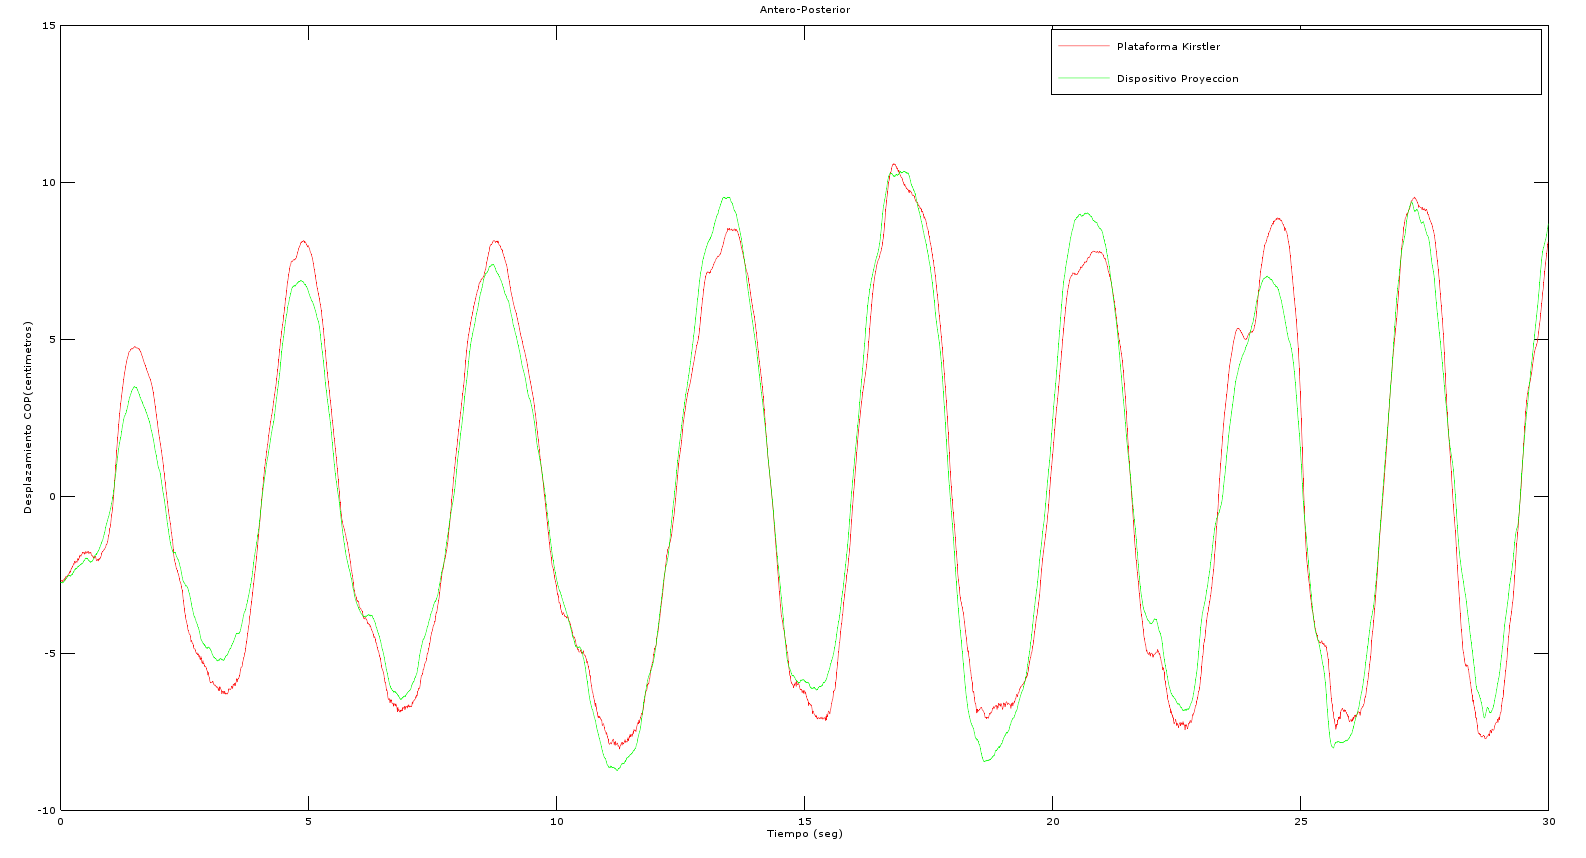
\includegraphics[scale=0.3]{images/Antero-PosteriorEspalda}
	\caption{Prueba Antero-Posterior Dispositivo Espalda}
	\label{fig:anteroPosteriorEspalda}
\end{figure}




\subsection{Principales Desafíos}
\subsubsection{Representación Tiempo Real}
La interfaz gráfica es una parte integral del sistema, pasando a ser la principal fuente de información para la retroalimentación, junto con el lugar donde mayormente interviene el usuario del sistema, entonces el no poder desplegar la información a tiempo, o que esta sea poco representativa es un gran problema. Se planteó inicialmente en graficar cada una de las salidas tanto del acelerómetro como el giroscopio en donde se representarían 6 variables según la frecuencia de muestreo, lo que en la práctica no resulta demasiado bien. Al representar en gráficos a frecuencias muy altas es decir 100hz o superior, multiplicado por la cantidad de datos que se estén representando, junto con el procesamiento interno para mostrar esos datos, se genera una sobrecarga en la parte gráfica, lo que conlleva a ralentizar el proceso, generando pérdidas de información y fidelidad al desplegar en tiempo real.

Para dar solución al problema, se implementó la opción de graficar un porcentaje de la información recibida en base a la frecuencia de muestreo seleccionada para la captura de información, con esto se asegura que la representación gráfica en tiempo real no sea un problema. Para ello a partir de la frecuencia de muestreo escogida para la prueba se calcula cada cuantas muestras debe ser enviado al gráfico principal, con el fin de no entorpecer la prueba ver Ecuación (\ref{eq:divisorFPS}), después de realizar el cálculo, del total de muestras obtenidas aplicando módulo del $DivisorFPS$, si el resultado del módulo es 0 se envía el dato.

Nota: Si la frecuencia de muestreo es menor a los FPS escogidos se enviarán todas las muestras considerando el resultado de la Ecuación (\ref{eq:divisorFPS}) = 1.

\begin{equation}
\label{eq:divisorFPS}
DivisorFPS=(int)\left(\frac{frecuenciaMuestreo}{FPS}\right)
\end{equation}

\subsubsection{Orientación Sensores}
Al momento de realizar la captura de información sensorial, junto con la obtención del ángulo de inclinación deben ser consideradas referenciado tales como:
\begin{itemize}
	
	\item \textbf{Referencia ejes del Sensores:} La obtención de información de aceleración y velocidad angular debe estar correctamente alineada con la referencia presente en los ejes del sensor, junto con la posición respecto al eje de gravedad de la tierra, para la correcta obtención de la información en base al movimiento ejercido por los sensores, y que estos sean descritos por los ejes que correspondan, para su posterior análisis o uso.
	
	\item \textbf{Posición en el Sujeto:} Junto con la referencia del sensor, se debe tomar en consideración en la posición que el prototipo o sistema final será puesta en el sujeto de estudio, ya que al cambiar la posición, las referencias internas del sensor dependen directamente de la posición, sino todo lo resultante va a cambiar, y con ello la información entregada comenzaría a describir el movimiento desde una perspectiva distinta a la planteada para los cálculos y estudio posterior.
\end{itemize}

Para dar solución a este inconveniente se incorporó en el software la opción de describir mediante la interfaz como será puesto el prototipo al momento de realizar las mediciones, usando un indicador de referencia clara, con el fin de no generar problemas para conocer la posición del sensor y facilitar al usuario final la tarea.
Según la orientación del sensor se generan distintas conjugaciones de los ejes a utilizar tanto para el cálculo del ángulo, como en el uso de la velocidad angular para la aplicación del filtro (en caso de ser utilizado), éstos se configuraron estudiando los ejes que debían ser usados según la orientación junto con el sentido en que varía la información de Acelerómetro y giroscopio, para así realizar el cálculo final.

\subsubsection{Data Terminal Ready}
Según el tipo de semiconductor del puerto USB de Arduino puede venir por defecto el Pin DTR (Data Terminal Ready) la función Reset de Arduino puede venir activada o desactivada. 
La función Reset de Arduino permite al microcontrolador reiniciar las variables internas según las configuraciones encontradas en el Setup del código de programación, para así eliminar cualquier cambio realizado en la ejecución del Loop,lo que es complicación al usar modelos de Arduino que tengan o no esta característica.

Para solucionar este problema se realiza una estandarización activando por Software el Pin DTR para que sin importar el modelo de semiconductor operen todos de forma igual en el software, para así no preocuparse de configuraciones o errores producidos debido al PIN DTR.

\subsubsection{Latencia en Controlador FTDI}
Por defecto el controlador del puerto USB FTDI para el Sistema Operativo Windows, en su configuración contenía una Latencia de 10 ms pre-configurada, lo que afecta considerablemente la captura de información sobre 100hz. El principal inconveniente que genero este error es la detección propia de éste, ya que al ser un error completamente aislado de los elementos que comúnmente son manipulados Arduino y Software, y a su vez es relativo a un modelo concreto de controlador de sistema y a su vez sistema operativo lo cual era de partida complejo de percibir y/o predecir.

La solución fue a partir de la información de configuración FTDI\cite{FTDI} para configurar directamente  en el registro de Windows (regedit) en la dirección asociada al controlador el parámetro de latencia deseado, para que éste sea lo más bajo posible.

\section{Conclusiones y Trabajos Futuros}
\subsection{Conclusiones}
\subsection{Trabajos Futuros}

\section{Bibliografía}
\printbibliography[heading=none]

\end{document}